\section{CH8 异常、调试与测试}

\begin{frame}[fragile]{CH8 异常、调试与测试}
  \begin{easylist} \easyitem
    & 异常
    && Python的异常处理使用方法
    && Python的异常继承关系
    && 利用raise抛出异常
    & 调试
    && print调试法
    && logging调试法
    && assert
    && pdb
    & 单元测试
  \end{easylist}
\end{frame}

\subsection{异常处理}
\subsubsection{异常处理使用方法}
\begin{frame}[fragile]{异常处理}
  \begin{easylist}
    & 程序在编写过程中,有大量情况需要考虑
    && 除数是否为0
    && 打开文件时,需要判断文件是否存在,有无权限
    && ...
    & 异常可以简化这一处理过程
    & Python的错误处理机制
    && try...except...finally...
  \end{easylist}
\end{frame}

\begin{frame}[fragile]{try}
  \begin{python}
try:
    print('try...')
    r = 10 / 0
    print('result:', r)
except ZeroDivisionError as e:
    print('except:', e)
finally:
    print('finally...')
print('END')    
  \end{python}

  try... \\
  except: division by zero \\
  finally... \\
  END \\
\end{frame}

\begin{frame}[fragile]{try}
  \begin{python}
try:
    print('try...')
    r = 10 / 2
    print('result:', r)
except ZeroDivisionError as e:
    print('except:', e)
finally:
    print('finally...')
print('END')    
  \end{python}

  try... \\
  result: 5.0 \\
  finally... \\
  END \\  
\end{frame}

\begin{frame}[fragile]{Python异常处理的规则}
  \begin{easylist}
    & 遇到第一个满足条件的异常,执行该异常下的语句,忽略后续的其它异常
    & finally永远会被执行
  \end{easylist}

\end{frame}

\subsubsection{异常继承关系}
\begin{frame}[fragile]{Python异常的继承关系}
  \begin{easylist}
    & Python的错误也是class,都继承自BaseException
    && 在使用except时需要注意的是,它不但捕获该类型的错误,还把其子类也“一网打尽”。
  \end{easylist}

  \begin{python}
lst = [x for x in range(10)]
try:
    n = lst[15]
except LookupError as e:
    print('LookupError ', e)
except IndexError as e:
    print('IndexError ', e)
  \end{python}
\end{frame}


\begin{frame}[fragile]{Python异常继承关系示例}
  \begin{center}
    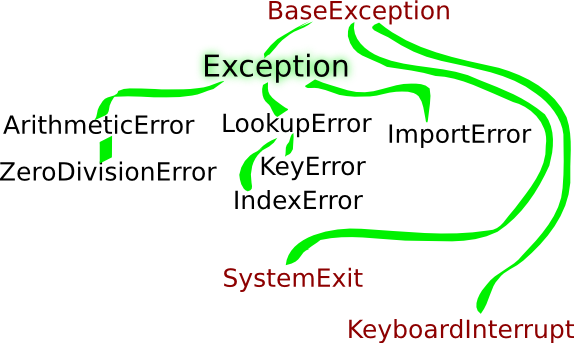
\includegraphics[width=0.8\textwidth]{figure/exception-hierarchy.png}
  \end{center}
  \url{https://docs.python.org/3/library/exceptions.html#exception-hierarchy}
\end{frame}

\subsubsection{利用raise抛出异常}
\begin{frame}[fragile]{抛出异常}
  \begin{easylist}
    & 可以用raise语句来引发一个异常。异常/错误对象必须有一个名字,且它们应是Error或Exception类的子类。
  \end{easylist}

\end{frame}


\begin{frame}[fragile, allowframebreaks]{raise示例}
  \begin{python}
class Student(object):
    |\color{red}@property|
    def score(self):
        return self._score

    |\color{red}@score.setter|
    def score(self, value):
        if not isinstance(value, int):
            raise ValueError('score必须是整数!')    
        if value < 0 or value > 100:
            raise ValueException('score必须在0到100之间')
        self._score = value   
\end{python}

\newpage
\begin{python}
s = Student()
s.score = 60
print(s.score)
|\color{red}s.score = 999| # Error!
\end{python}
\end{frame}


\begin{frame}[fragile, allowframebreaks]{异常可以自定义}
  \begin{easylist}
    & 例如:把以上的score判断条件不满足时,抛出的异常更改为自定义异常
  \end{easylist}

  \begin{python}
class ScoreException(Exception):
    def __init__(self, msg):
        self.msg = msg
        
    def __str__(self):
        return 'ScoreException: ' + repr(self.msg)
    
class Student(object):
    @property
    def score(self):
        return self._score

    @score.setter
    def score(self, value):
        if not isinstance(value, int):
            raise ScoreException('score必须是整数!')    
        if value < 0 or value > 100:
            raise ScoreException('score必须在0到100之间')
        self._score = value   
        
try:       
    s = Student()
    s.score = 60
    print(s.score)
    s.score = 999
except ScoreException as e:
    print(e)    
  \end{python}
\end{frame}

\begin{frame}[fragile]{异常总结}
  \begin{easylist}
    & Python内置的try...except...finally用来处理错误十分方便
    && 出错时,会分析错误信息并定位错误发生的代码位置更为关键
    & 程序也可以主动抛出错误,让调用者来处理相应的错误
    && 应在文档中写清楚可能会抛出哪些错误,以及错误产生的原因
  \end{easylist}
\end{frame}


\subsection{调试}
\begin{frame}[fragile]{调试}
  \large Bug and Debug
  \begin{columns}[onlytextwidth,T]
    \begin{column}{0.5\textwidth}
      \begin{block}{\small 格蕾丝·赫柏(Grace Murray Hopper)}
        \scriptsize{赫柏是一位为美国海军工作的电脑专家。1945年的一天,赫柏
        对Harvard Mark II设置好17000个继电器进行编程后,技术人员在进行整机运行时,
        它突然停止了工作。于是他们爬上去找原因,发现这台巨大的计算机内部一组继电
        器的触点之间有一只飞蛾,这显然是由于飞蛾受光和热的吸引,飞到了触点上,然
        后被高电压击死。所以在报告中,赫柏用胶条贴上飞蛾,并把“bug”来表示"一个在
        电脑程序里的错误"。}
      \end{block}
    \end{column}
    \begin{column}{0.45\textwidth}
      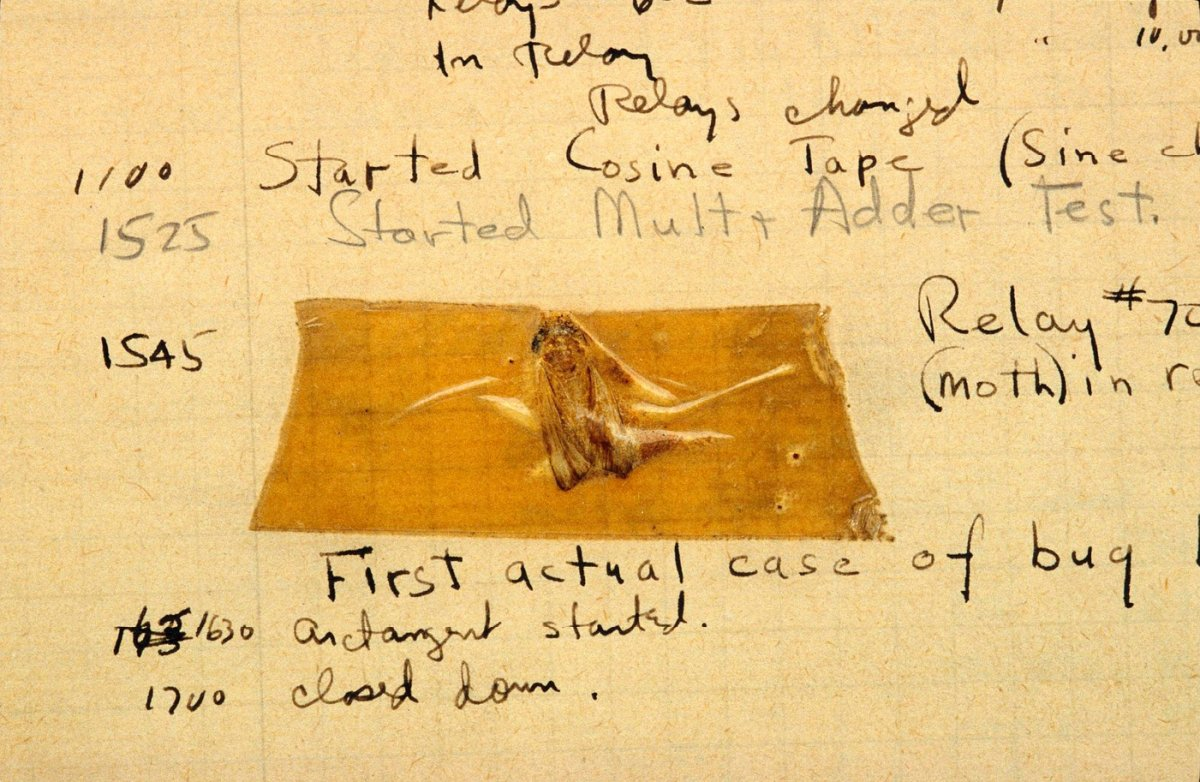
\includegraphics[width=0.85\textwidth]{figure/bug.jpg}
    \end{column}
  \end{columns}

  \begin{easylist}
    & 程序一次编写就能成功运行的概率很小,通常会有各种各样的错误需要调试,因此,
    掌握错误的调试方法非常重要。
  \end{easylist}
\end{frame}

\begin{frame}[fragile]{常用的调试方法}
  \begin{easylist}
    & 观察出错的提示信息
    & 利用print函数输出信息,观察输出结果和预期结果是否一致
    & 通过日志logging替代print
    & 利用assert断言
    & pdb
  \end{easylist}
\end{frame}

\subsubsection{利用print进行调试}
\begin{frame}[fragile]{利用print进行调试}
  \begin{python}
books = ['Python', 'XML', 'Information Retrieval']
for book in books:
    print(book)

print('Run here!') 
if book.price > 50:
    print('High price.')
  \end{python}

以上代码会抛出异常信息:

Traceback (most recent call last): \\
~~File "bug.py", line 5, in <module> \\
~~~~if book.price > 50: \\
AttributeError: 'str' object has no attribute 'price'\\

如果我们觉得前三行代码不太可能出问题,而问题很可能在后面,那我们可以在后面加入一
行print语句,观察程序能否正常运行到该位置,来缩小异常发生的范围
\end{frame}

\subsubsection{利用logging进行调试}
\begin{frame}[fragile]{利用logging进行调试}
  print()的结果默认输出到控制台上,不够灵活和方便,可以使用logging进行控制

  \begin{python}
import logging
logging.basicConfig(level=logging.INFO)

books = ['Python', 'XML', 'Information Retrieval']
for book in books:
    logging.info(book)

logging.debug('Run here!') 
if book.price > 50:
    logging.warn('High price.')
  \end{python}
\end{frame}

\subsubsection{assert调试}
\begin{frame}[fragile]{assert调试}
  assert断言用于判断给定的逻辑表达式是否成立,如果不成立,就会抛出AssertionError
  异常

\begin{python}
books = ['Python', 'XML', 'Information Retrieval']
assert len(books) == 3
\end{python}

启动Python解释器时可以用-O参数来关闭assert,此时的assert语句可看作是pass
\end{frame}

\subsubsection{pdb调试}
\begin{frame}[fragile]{pdb}
  Python的调试器,可以单步运行Python脚本,查看当前运行的代码,查看变量值

  bug.py: 
  \begin{python}
books = ['Python', 'XML', 'Information Retrieval']
for book in books:
    print(book)

if book.price > 50:
    print('High price.')
  \end{python}

  运行:pdb bug.py \\
  或者:python -m pdb bug.py

\end{frame}

\begin{frame}[fragile]{pdb}
  \begin{easylist}
    & n: 执行下一条语句
    & p xxx: 查看变量xxx的当前值
    & l: 列出
  \end{easylist}
\end{frame}

\begin{frame}[fragile]{pdb.set\_trace()}
  在可能出错的地方放置pdb.set\_trace(),程序运行到该条语句时,会暂停并进入pdb调试环
境,此时,可以用p指令查看变量,或者用c继续运行

  bug2.py: 
  \begin{python}
import pdb
books = ['Python', 'XML', 'Information Retrieval']
for book in books:
    print(book)

pdb.set_trace()
if book.price > 50:
    print('High price.')
  \end{python}
\end{frame}


\subsection{单元测试}
\begin{frame}[fragile]{单元测试}
  单元测试是用来对一个模块、一个函数或者一个类来进行正确性检验的测试工作。

\end{frame}


\begin{frame}[plain]{}
  \begin{center}
    ~ \\
    \Huge ---END---
  \end{center}
\end{frame}

%%% Local Variables:
%%% mode: latex
%%% TeX-master: "../python"
%%% End:
